\documentclass{jsarticle}
\bibliographystyle{ipsjunsrt.bst}
\usepackage[dvipdfmx]{graphicx, xcolor, hyperref}
\usepackage{amsmath}
\usepackage{amssymb}
\usepackage{bm}%太字ベクトル
\hypersetup{
    colorlinks=true,
    citecolor=blue,
    linkcolor=gray,
    urlcolor=blue
}
\title{計画ゼミ}
\author{後藤研 M1 三角}
\date{\today 更新}

\begin{document}
\maketitle

\tableofcontents

\section{2022年5月16日 第一回 ゼミ計画と線形計画法}

\subsection{ゼミ計画}

まず前提として過去問を入手していますよね?一応リンクを貼っておきます.

\url{https://drive.google.com/drive/folders/1I8odJc2l47IvJWGLyh4ZmIr2eZ5Tw6kh?usp=sharing}

\url{https://www.dropbox.com/sh/9sem7v37gpnvuia/AACnPxe8HZaPjIF7u20J7uyna?dl=0}

\url{https://www.dropbox.com/sh/lznmqg0bvjeiz50/AADgUeOOhITdNwE1h5wCDk6Na?dl=0}

予定通り進むか分かりませんがこのように全範囲を一周する予定です。
\begin{table}[htbp]
  \caption{ゼミの予定\label{table:plan}}
  \centering
  \begin{tabular}{ll}
    \hline
    日付 & 出題\\
    \hline \hline
    5/16&線形計画法\\
    6/1&非線形計画法\\
    6/6&費用便益分析、生産者行動・消費者行動\\
    6/13&動的計画法、PERT、重回帰分析\\
    \hline
  \end{tabular}
\end{table}

過去問の傾向をまとめました
\begin{table}[htbp]
  \caption{過去問傾向\label{table:kakomon}}
  \centering
  \begin{tabular}{ll}
    \hline
    年度 & 出題\\
    \hline \hline
    2021&非線形計画法、PERT(アローダイアグラム)\ref{pert2021} \\
    2020&線形計画法、費用便益分析\ref{costbenefit2020}\\
    2019&非線形計画法、重回帰分析\\
    2018&非線形計画法\ref{nonliner2018}、費用便益分析\\
    2017&線形計画法、動的計画法\\
    2016&交通計画、費用便益分析\\
    2015&非線形計画法、線形計画法・非線形計画法(定式化のみ)\\
    2014&非線形計画法、生産者行動・消費者行動\ref{action2014}、費用便益分析\\
    2013&重回帰分析\ref{jyukaiki2013}、PERT、動的計画法\ref{dynamic2013}\\
    2012&線形計画法、非線形計画法\\
    \hline
  \end{tabular}
\end{table}

出題範囲は狭く、計算も簡単なものが多いので計画理論は満点を狙いましょう.また簡単なので勉強時間は計画理論より土質や水理を優先した方が良いと思います.

\subsection{勉強方法}
過去問の問題と解答を10年分暗記しましょう.本番でも満点を狙えます.このゼミも過去問中心に進めます.質問も歓迎します
分からない部分は学部の教科書に載っています.

重回帰分析は数学の試験対策でも使える確率統計及び演習の教科書が便利です.
動的計画法は学部でやった記憶がないですが過去問URLの解答を見れば要領が掴めると思います.2016年の交通計画は問題文通りに立式すれば前提知識無しに解けるので対策は要らないと思います.

\begin{figure}[htbp]
  \begin{tabular}{c|c}
  藤井聡:土木計画学:2018&石倉智樹,横松宗太:公共事業評価のための経済学\\
  \hline
    
\includegraphics[keepaspectratio, width=5cm]{figures/doboku.png}
  &
    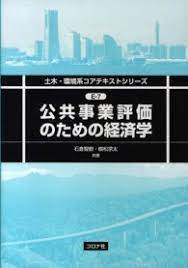
\includegraphics[keepaspectratio, width=5cm]{figures/kokyo.png}
  \\
  \begin{tabular}{l}社会システム計画論の教科書\\線形計画法\\非線形計画法\\PERT\end{tabular}
  &
  \begin{tabular}{l}公共経済学の教科書\\費用便益分析\\生産者行動・消費者行動\end{tabular}
  \end{tabular}
  \caption{参考文献\label{bibtext}}
\end{figure}

\subsection{線形計画法}

\begin{tabular}{c|c}
  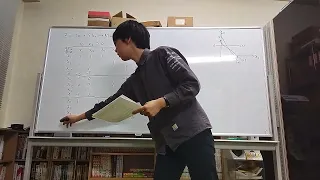
\includegraphics[keepaspectratio, width=3cm]{figures/0523.png}
  &
  \begin{tabular}{l}
  \url{https://youtu.be/PhPj25O_CIo}
  \\
  動画:20220516 計画ゼミ 線形計画法  2020年院試過去問解説
  \end{tabular}
\end{tabular}

\begin{figure}[htbp]
  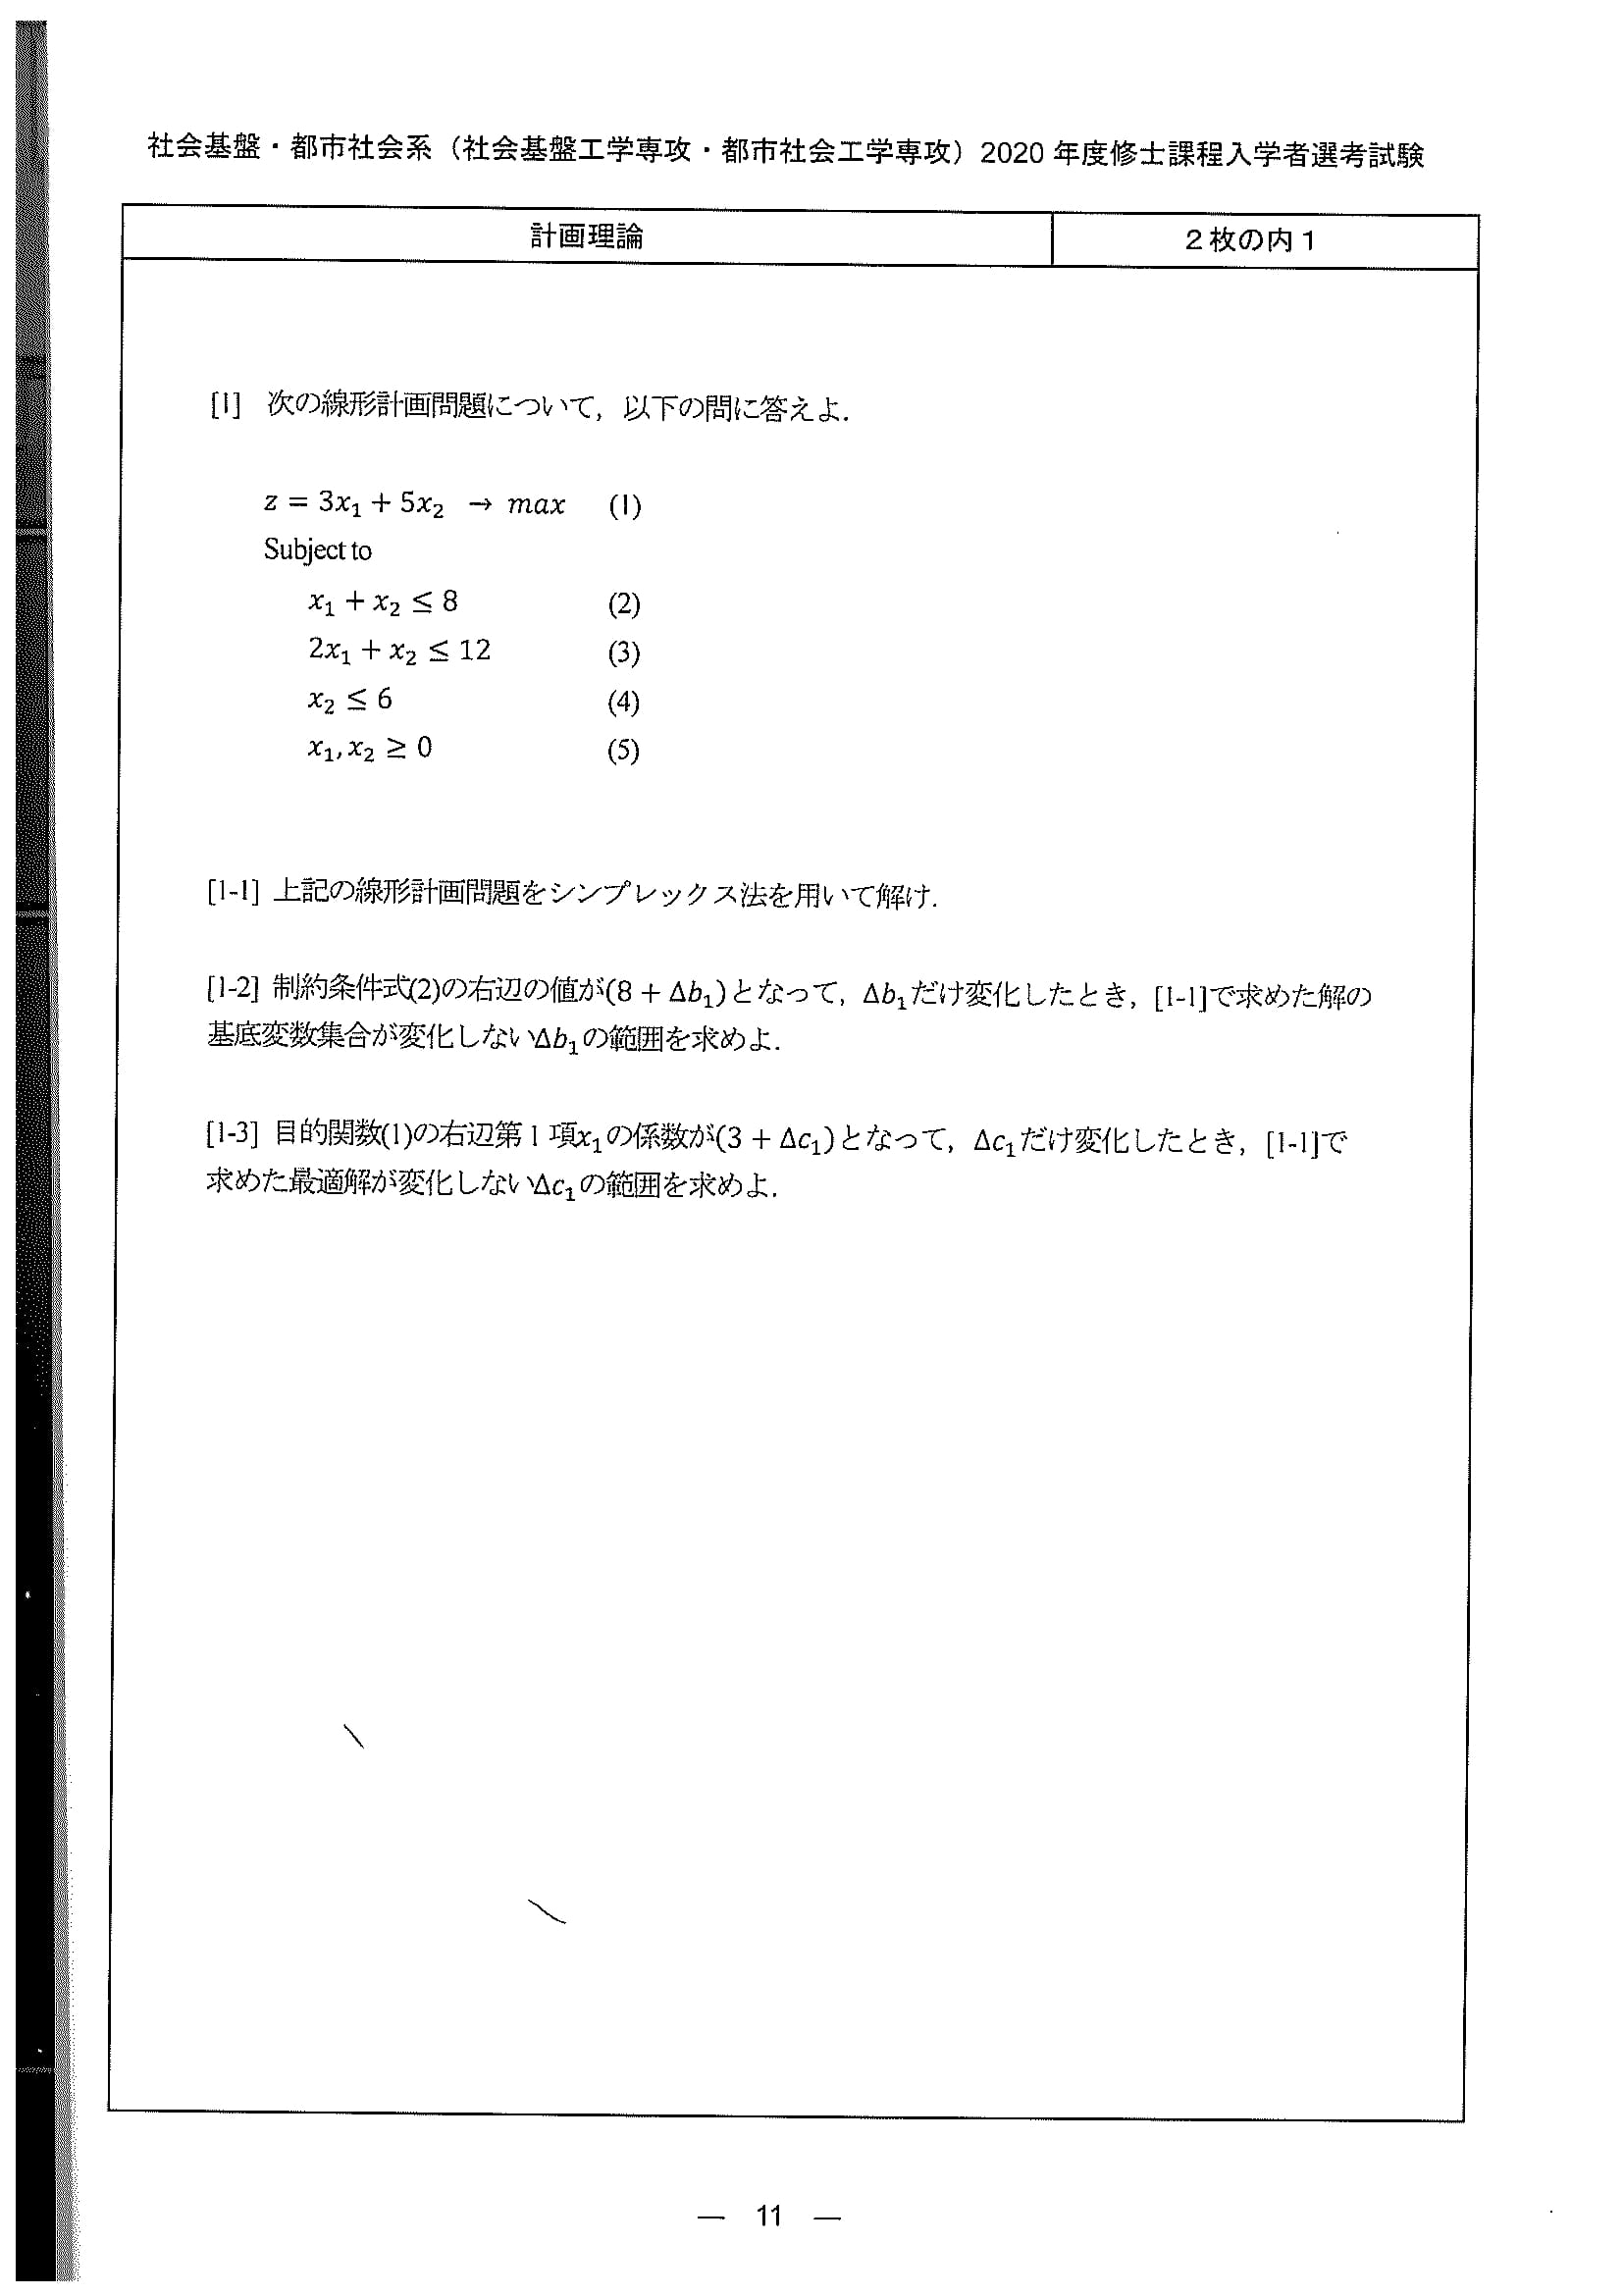
\includegraphics[keepaspectratio, width=16cm]{figures/liner2020.png}
  \caption{2020年線形計画法問題(動画解説済)\label{fig:liner2020}}
\end{figure}

アップロードするもの

・学部の社会システム計画論の線形計画法の演習pdfをアップロードします

・2020年の線形計画法(図\ref{fig:liner2020})を解く動画を今日中にアップロードします.

まずシンプレックスフローを反射神経でかけるように訓練してください、忘れてしまった人もいると思うので2020年の線形計画法を解く動画を今日中にアップロードします.
双対問題、感度分析は頻出なので復習しておいてください.感度分析は目的関数が変化するものと制約条件が変化するものの二種類が過去出題されています.

スラック変数は制約条件の限界からの余白を表しているので非負でないといけないとか、基底変数はシンプレックスフローの式中で唯一正の変数で他の変数はゼロであるとか、凸な多次元の多面体で表される実行可能領域を辺に沿って頂点から頂点へ解候補が移動し目的関数を最大化(最小化問題なら最小化)する頂点で停止するとかそういう概念を頭の中に描ければ完璧です.
増加限界が非負かつ最小な行について基底変数を入れ替える理由はそうでないと実行可能領域外に飛び出てしまうからです.

\begin{figure}[htbp]
  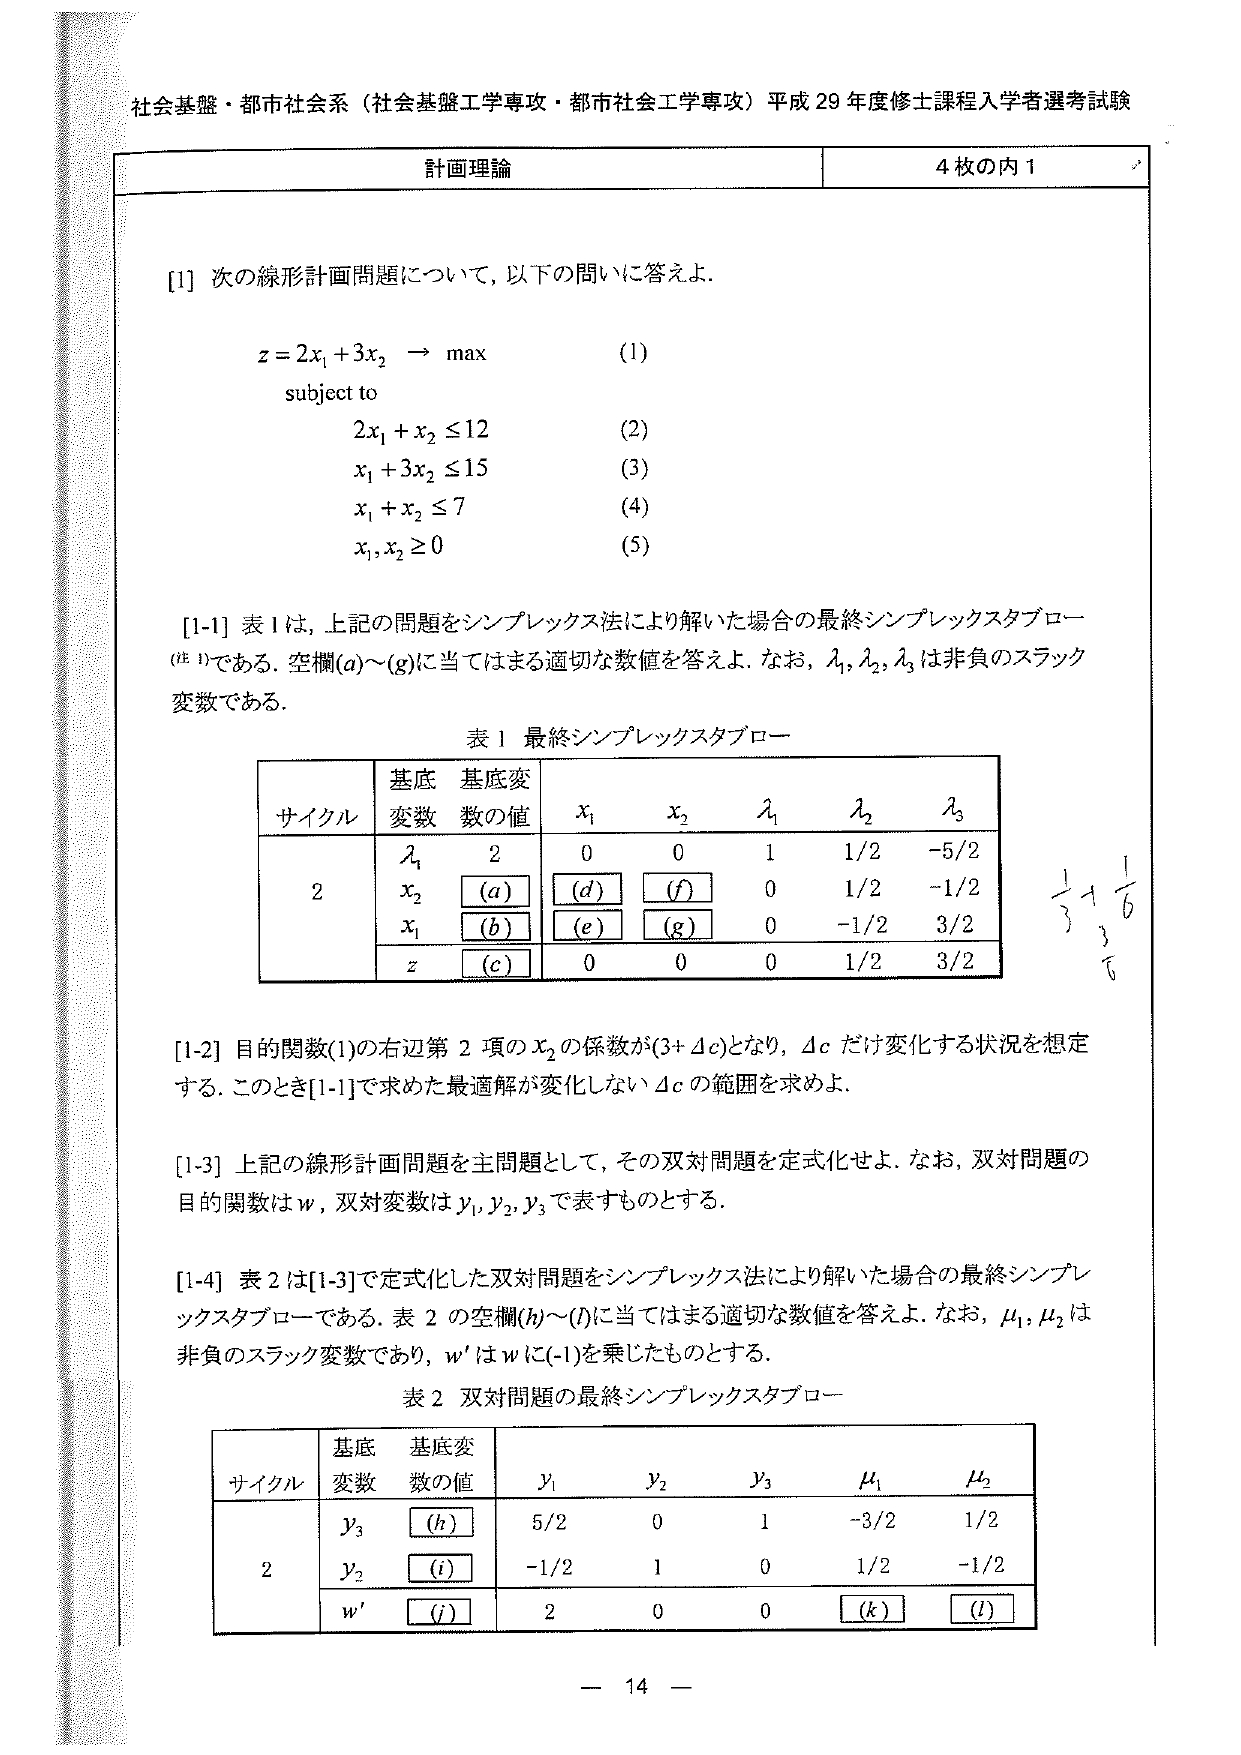
\includegraphics[keepaspectratio, width=16cm]{figures/liner2017.png}
  \caption{2017年線形計画法問題(課題)}
\end{figure}

\subsection{課題}
2017年の線形計画法(以下に記載)に自力で取り組み5/23(月)までに提出してください

今回は以上です.

\pagebreak
\section{2022年6月1日 第二回 非線形計画法:2018年過去問を例に解説\label{nonliner2018}}

\begin{tabular}{c|c}
  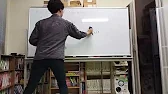
\includegraphics[keepaspectratio, width=3cm]{figures/0601.png}
  &
  \begin{tabular}{l}
  \url{https://youtu.be/6-CDAyntreU}
  \\
  動画:20220601 計画ゼミ 非線形計画法  2018年院試過去問解説
  図\ref{nonliner20181},図\ref{nonliner20182}参照
  \end{tabular}
\end{tabular}


本日は非線形計画法について説明します.2021,2019,2018,2015,2014,2012で出題されている頻出問題です。ここでは簡単な説明だけ書くので学部の教科書などで手順をしっかり学んでください。

非線形計画法の問題では凸計画問題であることを説明される場合が多いです.凸計画問題であることは目的関数$f$のヘッシアン行列$H(f)$が半正定であることで示せます、ヘッシアンはテンソル積で簡潔に書くとこうなり.

$$H(f)=\nabla \otimes \nabla f=
\begin{pmatrix}
\frac{\partial^2}{\partial x_1 \partial x_1} f & \frac{\partial^2}{\partial x_1 \partial x_2} f\\
\frac{\partial^2}{\partial x_2 \partial x_1} f & \frac{\partial^2}{\partial x_2 \partial x_2} f\\
\end{pmatrix}
$$

半正定とは行列式が非負のことです.

$$det(H(f))\ge0$$

次にラグランジュ関数を作ります。
不等式による制約条件を$g_k(\bm{x})\le0$の式に揃えます(kは不等式制約条件の番号)。

\begin{equation}
\begin{aligned}
x_1+x_2\le4 \\
x_1+x_2-4=g_k(\bm{x})\le0
\end{aligned}
\end{equation}

今回のように目的関数$f$の最小化問題ならばラグランジュ関数$L$は

$$L(\bm{x})=f(\bm{x})+\sum_k \lambda_k g_k(\bm{x})$$

最大化問題ならば

$$L(\bm{x})=f(\bm{x})-\sum_k \lambda_k g_k(\bm{x})$$

と設定します。符号に注意してください。

各$x_i$についてラグランジュ関数を偏微分し停留(定常性条件)で解を絞ります。

$$\frac{\partial L}{\partial x_1}=\frac{\partial L}{\partial x_2}=0$$

また各スラック変数$\lambda_k$についてラグランジュ関数を偏微分し制約条件を満たしている範囲(実行可能性)で解を絞ります。
$\lambda_k\ge0$は解が制約条件$k$で制約されていることを意味し$\lambda_k=0$は解が制約条件$k$に制約されていない(まだ余裕がある)ことを示します。
つまり前者なら$\frac{\partial L}{\partial \lambda_k}=g_k(\bm{x})=0$を,後者なら$\frac{\partial L}{\partial \lambda_k}=g_k(\bm{x})\le0$を満たす必要があります

\begin{align*}
\frac{\partial L}{\partial \lambda} = g(\bm{x})\le0 \;\text{and}\;\lambda=0
\\
\frac{\partial L}{\partial \lambda} = g(\bm{x})=0 \;\text{and}\;\lambda\ge0
\end{align*}

\begin{figure}[htbp]
  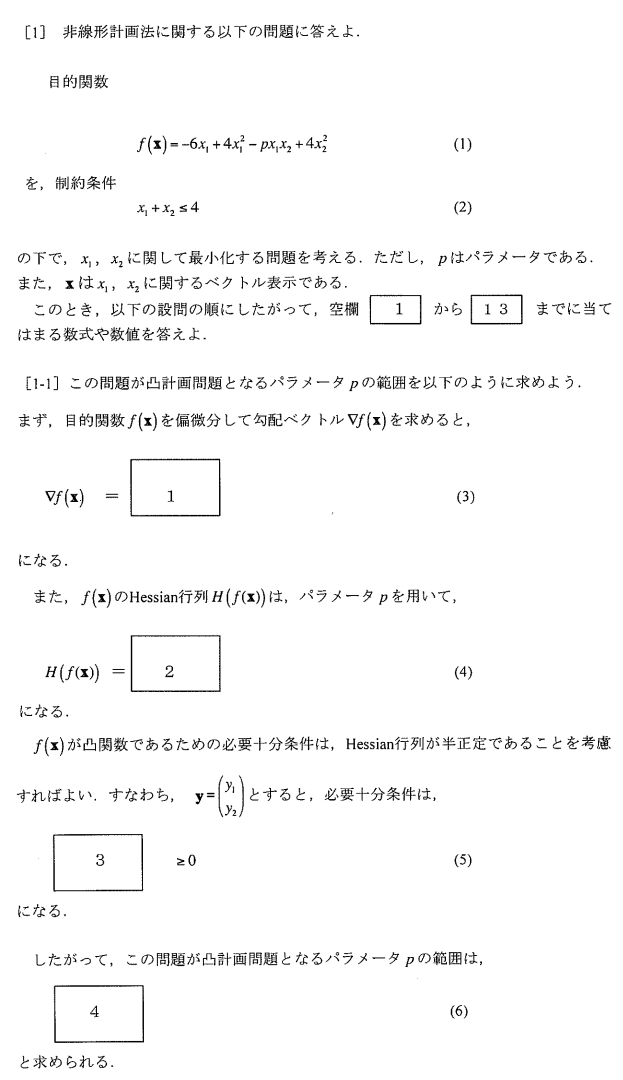
\includegraphics[keepaspectratio, width=14cm]{figures/nonliner2018.png}
  \caption{2018年非線形計画法問題1(動画解説済)\label{nonliner20181}}
\end{figure}

\begin{figure}[htbp]
  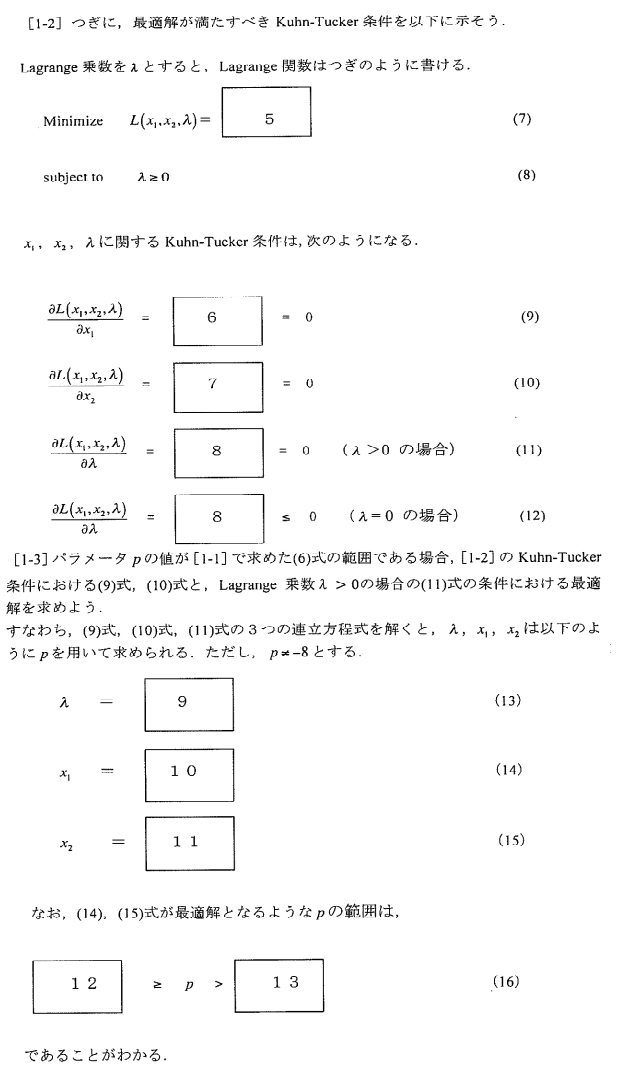
\includegraphics[keepaspectratio, width=14cm]{figures/nonliner20182.png}
  \caption{2018年非線形計画法問題2(動画解説済)\label{nonliner20182}}
\end{figure}


\subsection{課題}
2019年の非線形計画問題(図\ref{nonliner2019})を6/6月曜日までに解いてください。非線形計画法のなかでは簡単な問題だと思います。質問はLINEグループで24時間受け付けています。

\begin{figure}[htbp]
  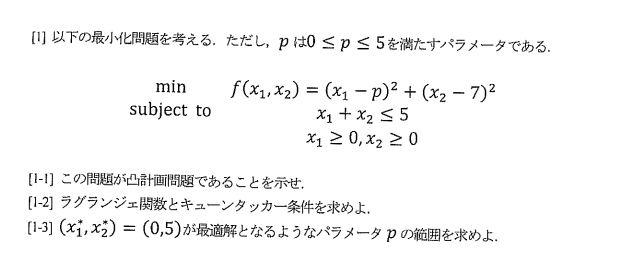
\includegraphics[keepaspectratio, width=16cm]{figures/nonliner2019.png}
  \caption{2019年線形計画法問題(課題)\label{nonliner2019}}
\end{figure}

\pagebreak
\section{2022年6月6日 第三回 費用便益分析と生産者行動・消費者行動}

課題は出しません,いつも通り勉強を進めてください。質問は受け付けています。個人LINEでもグループでもどうぞ。

\subsection{費用便益分析\label{costbenefit2020}}

費用便益分析はとても簡単で事業・プロジェクトへの投資額と利益の時系列から投資するべきかしないべきかを判断する手法です。院試問題を解くうえで必要な知識は少なく

$$B\textbf{便益(利益):benefit}=\sum_t \frac{b_t}{(1+r)^{t-1}}$$
$$C\textbf{費用:cost}=\sum_t \frac{c_t}{(1+r)^{t-1}}$$
のように将来の利益と費用の時系列を割引を加味した総額$B$,$C$に変換して考えます。ここに$t$:時間(多くは年),$r$:社会的割引率(年利のように,将来の利益や投資額を少なく見積もる率)です。

$B$と$C$を使って以下の三つの値を定義し,それらを見て投資するべきかしないべきかを判断します。

$$NPV\textmd{純現在価値}=B-C$$
NPV純現在価値は利益の規模を重視するときに使います。投資の回収の早さや,収益率は考慮しません。

$$CBR\textmd{費用便益比}=B/C$$
CBR費用便益比は費用に対して得られる利益の効率を重視します。利益の額は投資の回収の早さは考慮しません。

$$IRR\textmd{内部収益率}=r_{B=C}$$
IRR内部収益率は費用と利益が一致する場合の社会的割引率を指します。これは値が大きいほど早く投資を回収して利益を得られることを意味します。

2020年の費用便益分析の問題が解ければ他の年度の類似問題も解けると思います.

\begin{figure}[htbp]
  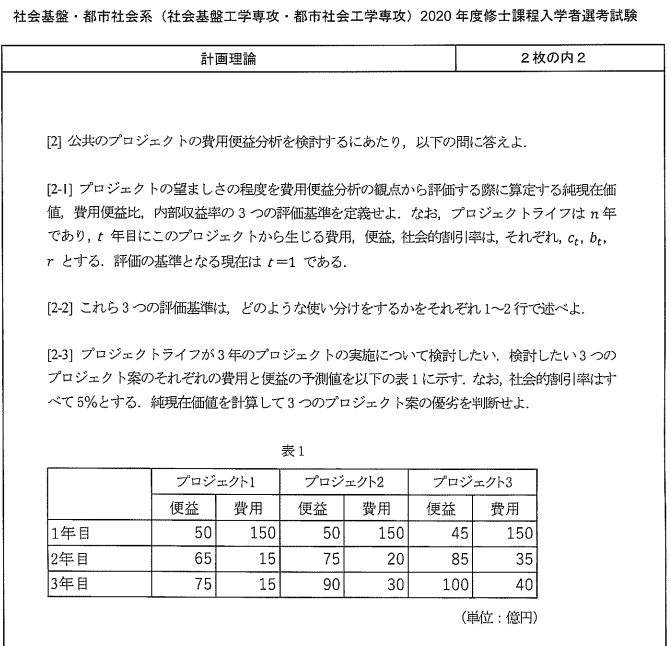
\includegraphics[keepaspectratio, width=16cm]{figures/costbenefit2020.png}
  \caption{2020年費用便益分析\label{costbenefit20201}}
\end{figure}


\subsection{生産者行動・消費者行動:2014年過去問を例に\label{action2014}}

2014年に少し出た問題です.出題頻度は高くないと思います.公共経済学の教科書を見れば解けると思います。

\begin{figure}[htbp]
  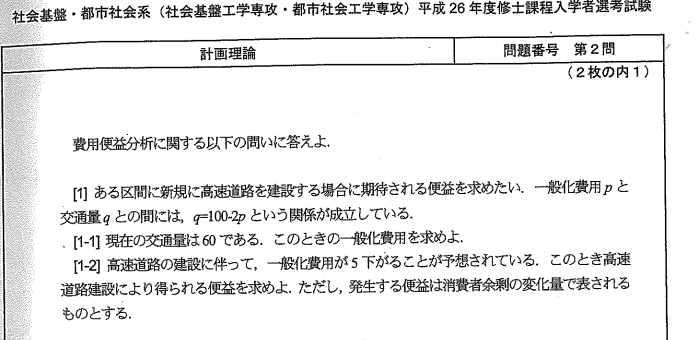
\includegraphics[keepaspectratio, width=16cm]{figures/costbenefit2014.png}
  \caption{2014年生産者行動・消費者行動\label{action20141}}
\end{figure}

2014年の問題は一般化費用$p$と交通量$q$と提示されていますが$q$が価格により決まる需要関数と見なせば
1-1は$60=100-2p$より$p=20$,一般化費用$p$が5下がるといわれているので$p=20$から$p=15$までの消費者余剰の変化量は
$$\int_15^20 q dp=\int_15^20 (100-2p) dp=325$$
と求まります。

\subsection{生産者行動・消費者行動の資料(昔のレポート)}

ある財の需要関数と供給関数がそれぞれ
$d-392-p, s=p-14$
で示されるとする.
この財に3\%の消費税が課せられたする.

\paragraph{課税前の均衡価格と取引量を求めよ.}

$d=s$より,価格$p=203$,取引量$d=s=189$

\paragraph{消費税導入における消費者余剰と生産者余剰の損失を求めよ.}
消費価格$p_d$と生産価格$p$の関係は$p_d=1.03p$
需給のつりあいより$392-p_d=p-14$,従って$p=200$,$p_d=206$,取引量$s=s=186$

消費者余剰$CS$は
$$CS=\int_{203}^{206} d \cdot d p_d=\frac{(186+189)(206-203)}{2}=562.5$$
生産者余剰$PS$は
$$PS=\int_{200}^{203} d \cdot d p=\frac{(186+189)(203-200)}{2}=562.5$$

\paragraph{政府の税収と課税によって発生する社会的余剰の損失を求めよ.}

税収は$0.03\times186\times200=1116$
社会的余剰の損失は$PS+CS-\textmd{税収}=562.5+562.5-1116=9$

\paragraph{二財$x$,$y$と二個人A, B からなる純粋交換経済において,各個人の効用関数と財の初期保有量がそれぞれ,$u^A=x^2y$,$u^B=xy^2$,$(x^A,y^A)=(90,0)$,$(x^B,y^B)=(0,60)$
で示されるとする
}

\paragraph{個人 A, Bの超過需要を求めよ.}
個人Aの効用最大化問題は

$\max u^A=x^2y$ s.t. $p_x x+p_y y= 90 p_x$

ラグランジュの未定乗数法より

$\nabla (x^2 y)=\lambda \nabla (p_x x+p_y y - 90 p_x)$かつ
$p_x x+p_y y - 90 p_x=0$

これを解いて$x^A=60$,$y^A=30\frac{p_x}{p_y}$

個人Aの超過需要は$(ED_x^A,ED_y^A)=(60-90,30\frac{p_x}{p_y}-0)=(-30,30\frac{p_x}{p_y})$

個人Bの効用最大化問題は

$\max u^A=xy^2$ s.t. $p_x x+p_y y= 60 p_y$

ラグランジュの未定乗数法より

$\nabla (xy^2)=\lambda \nabla (p_x x+p_y y - 60 p_y)$かつ
$p_x x+p_y y - 60 p_y=0$

これを解いて$x^A=20\frac{p_y}{p_x}$,$y^A=40$

個人Bの超過需要は$(ED_x^A,ED_y^A)=(20\frac{p_y}{p_x},40-60)=(20\frac{p_y}{p_x},-20)$

\paragraph{ワルラス均衡における二財の価格比を求めよ.また,均衡では二個人はどのような取引を行うか.}

ワルラス均衡では全ての財について超過需要の総和が0である
$$ED_x^A+ED_x^B=ED_y^A+ED_y^B=0$$
これを解いて価格比は
$$\frac{p_x}{p_y}=\frac{2}{3}$$
近郊ではAはyを20個買い,Bはxを30個買うように取引する.

\textbf{ある独占企業の逆需要関数が$p(y)=150-y$、費用関数が$c(y)=50y+900$ で与えられていたとする。}

\paragraph{この企業が利潤最大化をする場合の供給量、価格、利潤、消費者余剰、生産者余剰、総余剰を求めよ。}

限界費用$MC=c'(y)=50$かつ限界収入$MR=\frac{d(yp(y))}{dy}=150-2y$.
利潤最適化する場合$MR=MC$または$\frac{d\pi}{dy}=0$より供給量$y=50$,価格は$p(50)=100$,利潤は$\pi(y)=yp(y)-c(y)$,$\pi(50)=1600$

消費者余剰は$$CS=\int_0^{50} p(y) dy - 100\cdot 50=1250$$

生産者余剰は$$PS=100 \cdot 50 - \int_0^{50} c'(y) dy - 100\cdot 50=2500$$

総余剰は$1250+2500=3750$

\paragraph{この企業が政府から限界費用料金規制を受けた場合の供給量、価格、利潤、消費者余剰、生産者余剰、総余剰を求めよ。}

$p=c'(y)=50$となる.
供給量は$y=150-p=100$.
利潤は$\pi=50\cdot100-50\cdot100-900=-900$.

消費者余剰は逆需要関数の積分から支払額を引いて
$$CS=\int_0^{100} p(y) dy - 100\cdot 50=5000$$
生産者余剰は
$$PS=50 \cdot 100 - \int_0^{100} c'(y) dy =0$$
総余剰は$TS=5000+0=5000$

\paragraph{この企業がから平均費用料金規制を受けた場合の供給量、価格、利潤、消費者余剰、生産者余剰、総余剰を求めよ。}

平均費用料金規制より
$$p=\frac{c(y)}{y}$$
これをといて
$$50+\frac{900}{y}=150-y$$
より余剰が大きくなる大きい方の解を採用し
$$y=90$$

このときの価格と利潤は

$p(y)=150-90=60$,$\pi=p(y)y-c(y)=60\cdot90-50\cdot90-900=0$

消費者余剰は

$$CS=\int_0^{90}py(y)dy-60\cdot90=4050$$

生産者余剰は

$$PS=60\cdot90-\int_0^{90}c'(y)dy=900$$

総余剰は

$$TS=CS+PS=4050+900=4950$$

\textbf{ある工場では平均費用と限界費用が等しく、生産一単位あたり 200 万円であるとする。この工場の生産物に関する需要は下記の需要関数$Q( p) =1000 − p$で表される( p の単位:万円)。一方工場の近隣住民は大気汚染や汚染物質の排水などで外部不経済をこうむる。この外部費用は生産一単位あたり 100 万円とする。}

\paragraph{a. 政府が外部不経済を放置しているとき、決定される供給量と価格を求めよ}

$MC=200$かつ$MR=\frac{d p(y)y}{dy}=1000-2y$

従って供給量は$y=400$,価格は$p=600$

\paragraph{b. 均衡において生産物需要者に帰属する消費者余剰と近隣住民に帰属する外部費用の金額を求めよ。}

消費者余剰は$\frac{(1000-600)\cdot400}{2}=80000$,外部費用は$100y=40000$

\paragraph{c. 政府が企業に対して生産一単位あたり 100 万円税金をかけるとき、均衡における供給量と価格を求めよ。}

$MC=200+100$として$MR=MC$より供給量$y=350$,価格$p=650$

\paragraph{d. cの均衡における消費者余剰、外部費用、税収をそれぞれ求めなさい}

消費者余剰$CS=\frac{(1000-650)\cdot350}{2}=61250$,
外部費用$350\cdot100=35000$,
税収$350\cdot100=35000$

\section{2022年6月26日 第四回 動的計画法、PERT、重回帰分析}

\subsection{動的計画法 2013年度過去問\label{dynamic2013}}

動的計画法とは時間的広がりを持つ(=動的(Dynamic))問題を扱う最適化手法です。複雑な問題を時間軸上の複数の簡単な問題に分解し解いていきます。2017年度の過去問では長期間の道路整備費用を最小化する問題を第$i$期末以降の費用を最小化する整備行動を選択する問題に落とし込んでいます。2013年度の過去問では季節商品の利益を最大化する問題を第$i$期以降の利益を最大化する最適な発注・販売計画を選択する問題に落とし込んでいます。いずれも未来の目的関数を用いて現在の目的関数を導く漸化式を作っている点,目的関数は現在以降の総利益や現在以降の総費用等の現在以降の何らか値の総和を表す関数である点に注目してください。動的計画法はそのように設定した目的関数を各段階で最大化または最小化します。


\begin{figure}[htbp]
  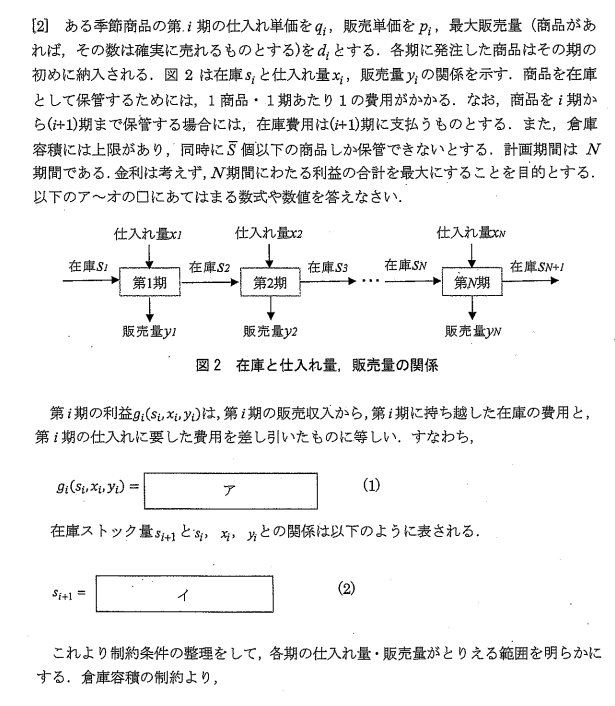
\includegraphics[keepaspectratio, width=16cm]{figures/dynamic20131.png}
  \caption{2013年動的計画法1枚目\label{dynamic20131}}
\end{figure}

\pagebreak

上記を意識したうえで誘導に乗って解答しましょう
\paragraph{ア.「第$i$期の利益$g_i(s_i,x_i,y_i)$は第$i$期の販売収入から,第$i$期に持ち越した在庫の費用と第$i$期の仕入れに要した費用を差し引いたものに等しい」は以下のように立式できます$$g_i(s_i,x_i,y_i)=p_i\cdot y_i-s_i-q_i\cdot x_i$$}
\paragraph{イ.在庫ストック量は前後の在庫の差分が販売量-仕入れ量になるので$$s_{i+1}=s_i+x_i-y_i$$}
\paragraph{ウ.「販売量はその期の在庫$s_i$と仕入れ量の$x_i$の和を上回ることはできない」つまり無いものは売れないことを立式して$$0 \ge y_i \ge s_i+x_i$$}
\paragraph{エ.文意を汲むと次期の在庫が保管限界量に達しない条件$0\ge s_{i+1} \ge \overline{S}$に$s_{i+1}=s_i+x_i-y_i$を代入して
\begin{align*}
0 \ge s_i+x_i-y_i \ge \overline{S} \therefore
\\
y_i-s_i \ge s_i \ge \overline{S}+y_i-s_i
\end{align*}}

ここまでは誘導に乗るだけです.以下の解答は最初に説明した動的計画法を知らないと難しいです。

\begin{figure}[htbp]
  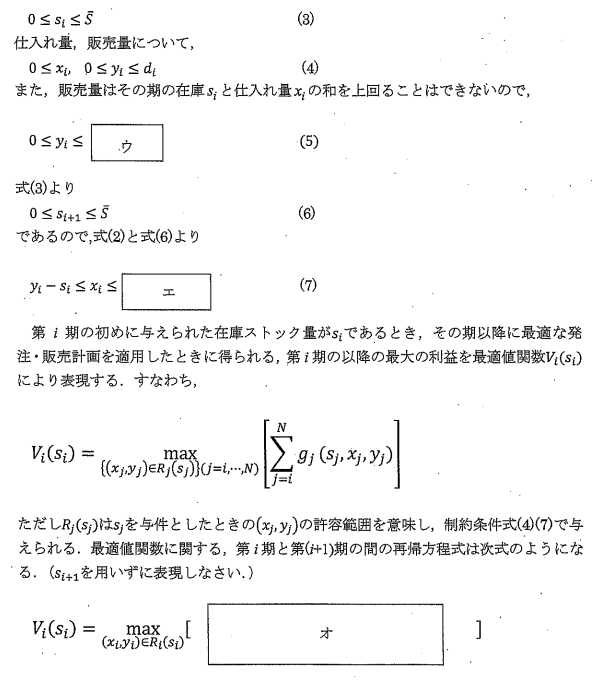
\includegraphics[keepaspectratio, width=16cm]{figures/dynamic20132.png}
  \caption{2013年動的計画法2枚目\label{dynamic20132}}
\end{figure}

\pagebreak

\paragraph{オ.文章中の最適地関数$V_i(s_i)$はこの問題の目的関数です。「その期以降に最適な発注・販売計画を適用したときに得られる,第$i$期の以降の最大の利益」と丁寧に説明されているのでこの目的関数を最大化すれば良いのです。未来の目的関数で現在の目的関数を表すという動的計画法の特徴から
\begin{align*}
V_i(s_i)=\underset{\{(x_j,y_j)\in \bm{R}_j(s_j)\}(j=i,\cdots,N)}{\max}\left[\sum_{j=i}^N g_j(s_j,x_j,y_j)\right]
\end{align*}
ここで最大化の中身は以下のように分解できます。
\begin{align*}
\sum_{j=i}^N g_j(s_j,x_j,y_j)=g_i(s_i,x_i,y_i) +\sum_{j=i+1}^N g_j(s_j,x_j,y_j)=g_i(s_i,x_i,y_i)+V_{i+1}(s_{i+1})
\end{align*}
よって以下のように漸化式が求まります。
\begin{align*}
V_i(s_i)=\underset{(x_i,y_i)\in \bm{R}_i(s_i)}{\max}\left[g_i(s_i,x_i,y_i)+V_{i+1}(s_{i+1})\right]
\end{align*}}

\subsection{PERT 2021年度過去問\label{pert2021}}

2021の過去問の解答を見れば大体分かると思います。文章で説明しずらいところが有ったので私が問題用紙に書き込みました。トータルフローとフリーフローの違いは分かってない人も多いと思うので図\ref{pert20211}の右下の簡単に解説しました。復習しておいてください

\begin{figure}[htbp]
  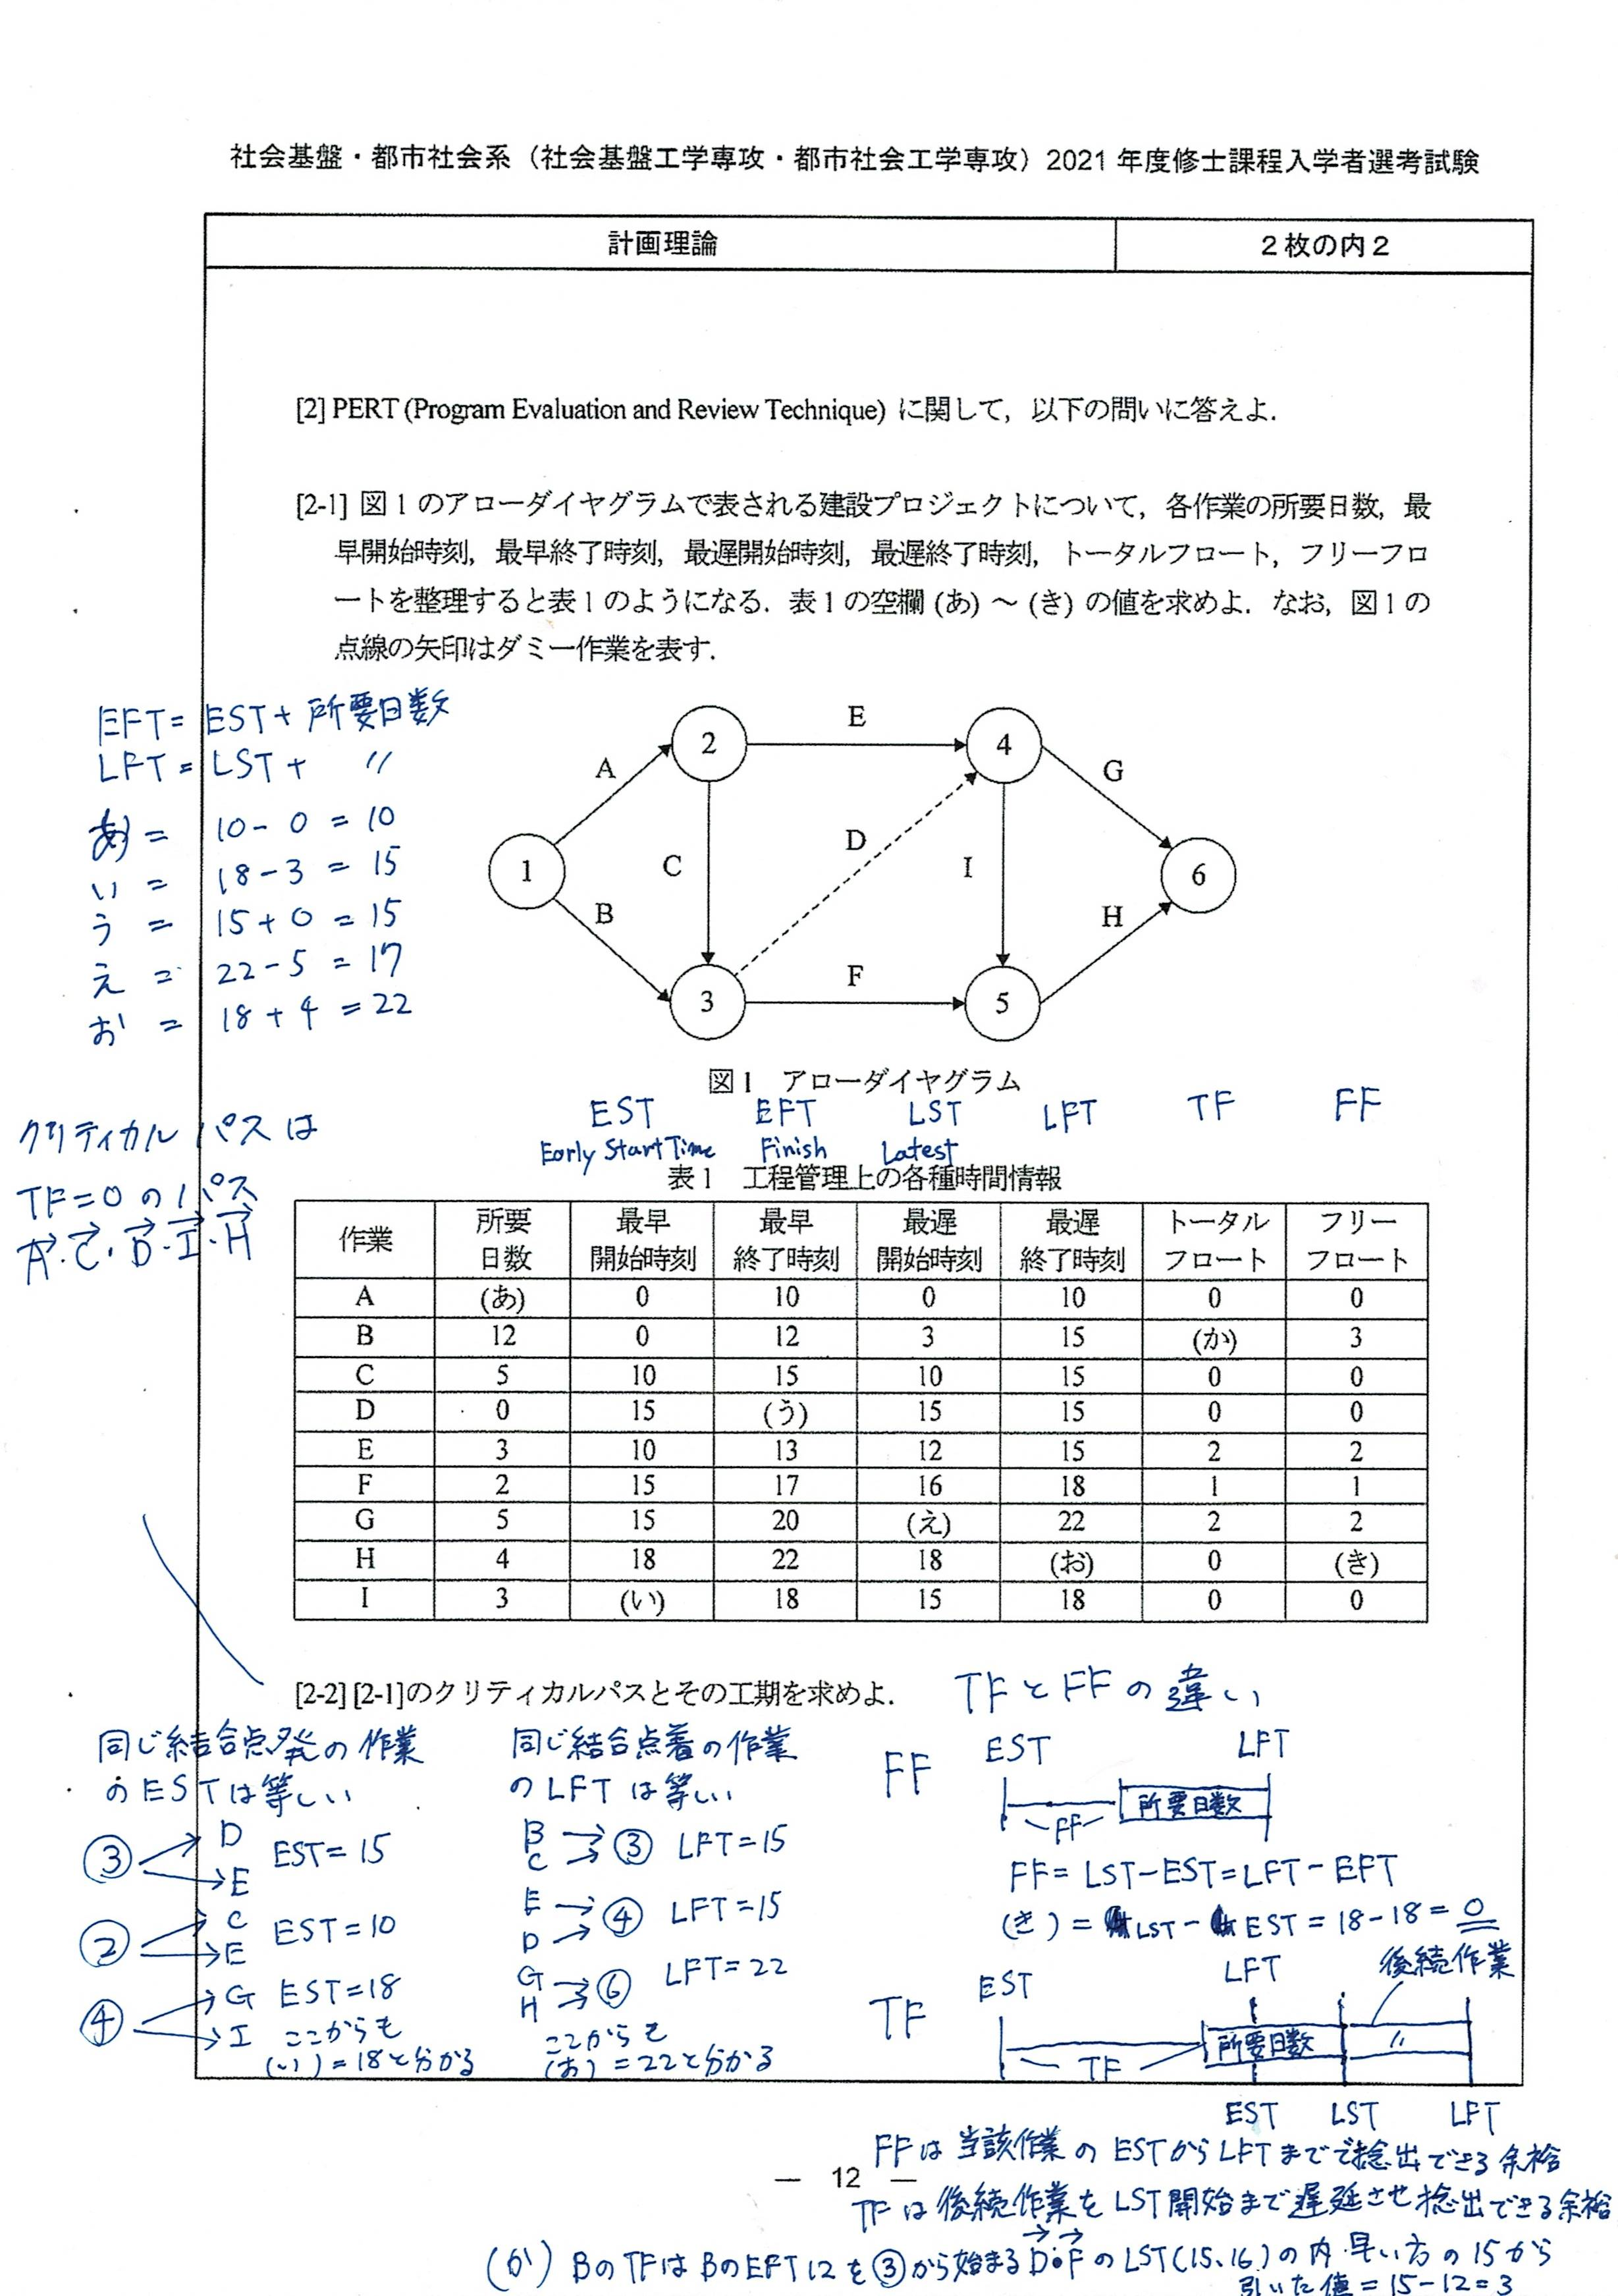
\includegraphics[keepaspectratio, width=16cm]{figures/pert20211.jpg}
  \caption{2021年PERT1枚目\label{pert20211}}
\end{figure}

\pagebreak

\subsection{重回帰分析 2013年度過去問\label{jyukaiki2013}}

重回帰分析は被説明変数$y_i$の予測値$\hat{y}_i$を複数の説明変数$x_{ji}$と係数$\beta_j$の線形方程式で表すとして、誤差$\epsilon_i$の二乗の総和を最小化する係数$\beta_i$を求める分析です。

$$\hat{y}_i=\beta_0+\beta_1 x_{1i}+\beta_2 x_{2i}+\beta_3 x_{3i}+\beta_4 x_{4i}+\beta_5 x_{5i}\cdots$$
$$y_i=\beta_0+\beta_1 x_{1i}+\beta_2 x_{2i}+\beta_3 x_{3i}+\beta_4 x_{4i}+\beta_5 x_{5i}\cdots+\epsilon_i=\hat{y}_i+\epsilon_i$$
院試では人口と土地面積からGDPを推定するなどの過去問が出題されていますし,私三角の卒論では歩行速度$[m/s]$と水深$[m]$(説明変数)から流体力$[N]$を推定しました。(そのまま重回帰分析すると係数$\beta_i$に単位が付き比較しにくいので説明変数・被説明変数共に無次元化しています)

係数$\beta_i$は二乗誤差$\epsilon^2=(y-\hat{y})^2$の総和の最小化問題$\text{minimize}\;\sum \epsilon^2$を解いて求めます。
非線形計画法として考えると二乗誤差の総和は最小化すべき目的関数であり(制約条件が無いので)ラグランジュ関数でもあります。
$\beta_i$の二次関数なので凸関数であり解けます。停留点の条件は以下の連立方程式になります。

$$\frac{\partial L}{\partial \beta_i}=\frac{\partial  \sum \epsilon^2}{\partial \beta_i}=\frac{\partial  \sum (y-\hat{y})^2}{\partial \beta_i}=0$$
これを正規方程式(normal equations)と呼び,これを解いて係数$\beta_i$が求まります。
2013年の重回帰分析の過去問を解きながら解説していきます。

\begin{figure}[htbp]
  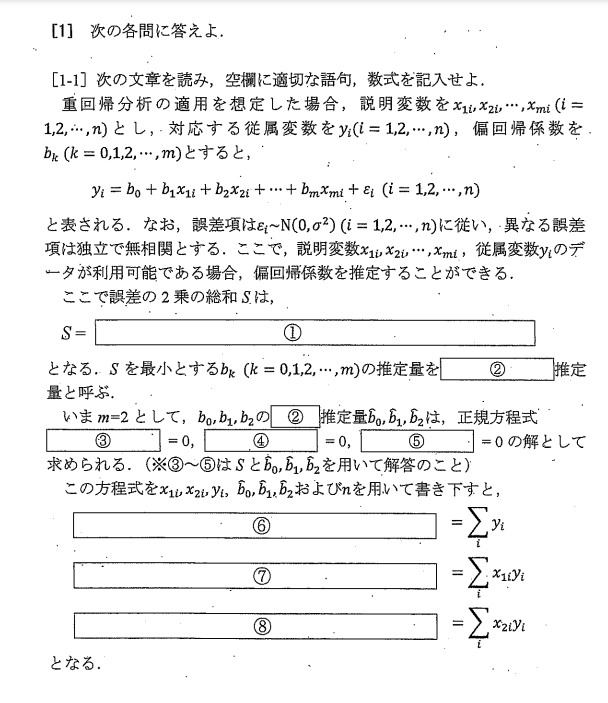
\includegraphics[keepaspectratio, width=16cm]{figures/jyukaiki20131.png}
  \caption{2013年重回帰分析1枚目\label{jyukaiki20131}}
\end{figure}

\pagebreak

1.二乗誤差の総和$S$の定義なので
$$S=\sum \epsilon_i^2=\sum \left\{y_i-(b_0+b_1 x_{1i}+b_2 x_{2i}+\cdots+b_m x_{mi})\right\}^2$$

2.$b_i$の推定値(正規方程式を解いて求めた値)を最尤推定量$\hat{b}_i$と呼びます

3.4.5.正規方程式の定義より
\begin{align*}
\frac{\partial S}{\partial \hat{b}_0}&=0&\frac{\partial S}{\partial \hat{b}_1}&=0&\frac{\partial S}{\partial \hat{b}_2}&=0
\end{align*}

6.二乗誤差の総和$S$を代入して整理
\begin{align*}
\frac{\partial S}{\partial \hat{b}_0}&=\sum_i \frac{\partial \left\{y_i-(\hat{b}_0+\hat{b}_1 x_{1i}+\hat{b}_2 x_{2i})\right\}^2}{\partial \hat{b}_0}=\sum_i 2\left\{y_i-(\hat{b}_0+\hat{b}_1 x_{1i}+\hat{b}_2 x_{2i})\right\}\cdot-1=0
\\
 \therefore \sum_i y_i &= \sum_i \left\{\hat{b}_0+\hat{b}_1 x_{1i}+\hat{b}_2 x_{2i}\right\}=n\hat{b}_0+\hat{b}_1 \sum_i x_{1i}+\hat{b}_2 \sum_i x_{2i}
\end{align*}

7.二乗誤差の総和$S$を代入して整理
\begin{align*}
\frac{\partial S}{\partial \hat{b}_1}&=\sum_i \frac{\partial \left\{y_i-(\hat{b}_0+\hat{b}_1 x_{1i}+\hat{b}_2 x_{2i})\right\}^2}{\partial \hat{b}_1}=\sum_i 2\left\{y_i-(\hat{b}_0+\hat{b}_1 x_{1i}+\hat{b}_2 x_{2i})\right\}\cdot-x_{1i}=0
\\
 \therefore \sum_i x_{1i} y_i &= \sum_i \left\{\hat{b}_0+\hat{b}_1 x_{1i}+\hat{b}_2 x_{2i}\right\}x_{1i}=\hat{b}_0\sum_i x_{1i}+\hat{b}_1 \sum_i x_{1i}^2+\hat{b}_2 \sum_i x_{1i} x_{2i}
\end{align*}

8.二乗誤差の総和$S$を代入して整理
\begin{align*}
\frac{\partial S}{\partial \hat{b}_2}&=\sum_i \frac{\partial \left\{y_i-(\hat{b}_0+\hat{b}_1 x_{1i}+\hat{b}_2 x_{2i})\right\}^2}{\partial \hat{b}_2}=\sum_i 2\left\{y_i-(\hat{b}_0+\hat{b}_1 x_{1i}+\hat{b}_2 x_{2i})\right\}\cdot-x_{2i}=0
\\
 \therefore \sum_i x_{2i} y_i &= \sum_i \left\{\hat{b}_0+\hat{b}_1 x_{1i}+\hat{b}_2 x_{2i}\right\}x_{2i}=\hat{b}_0\sum_i x_{2i}+\hat{b}_1 \sum_i x_{1i} x_{2i}+\hat{b}_2 \sum_i x_{2i}^2
\end{align*}

\begin{figure}[htbp]
  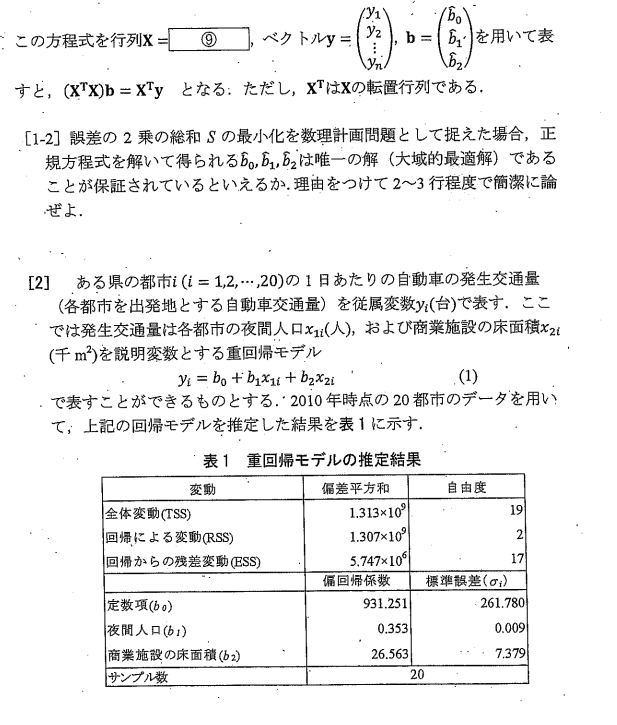
\includegraphics[keepaspectratio, width=16cm]{figures/jyukaiki20132.png}
  \caption{2013年重回帰分析2枚目\label{jyukaiki20132}}
\end{figure}

\pagebreak

9.これは正規方程式6,7,8が$(\bm{X}^T \bm{X})\bm{b}=\bm{X}^T \bm{y}$で書けるとすると$\bm{X}^T \bm{y}$が6,7,8の$\sum_i y_i$,$\sum_i x_{1i} y_i$,,$\sum_i x_{1i} y_i$に相当すると考えられ,比較から$\bm{X}$を以下のように置くと正規方程式と$(\bm{X}^T \bm{X})\bm{b}=\bm{X}^T \bm{y}$が一致します.\emph{出回っている解答は間違っているので注意してください、私の解答の方が正しいはずです}

\begin{align*}
\bm{X}=\begin{bmatrix}
1 & x_{11} & x_{21}\\
1 & x_{12} & x_{22}\\
\vdots & \vdots & \vdots \\
1 & x_{1n} & x_{2n}
\end{bmatrix}
\end{align*}

[1-2].誤差の二乗の総和$S$の最小化について正規方程式を解いて得られる解$\hat{b}_0,\hat{b}_1,\hat{b}_2$が大域的最適解である理由は$S$が$\hat{b}_0,\hat{b}_1,\hat{b}_2$の凸関数であり,その最小化は凸計画問題なので局所的最適解と大域的最適解が一致するからです。非線形計画法や線形計画法で説明したのと同じ文言を書けば点数が来ると思います。

\begin{figure}[htbp]
  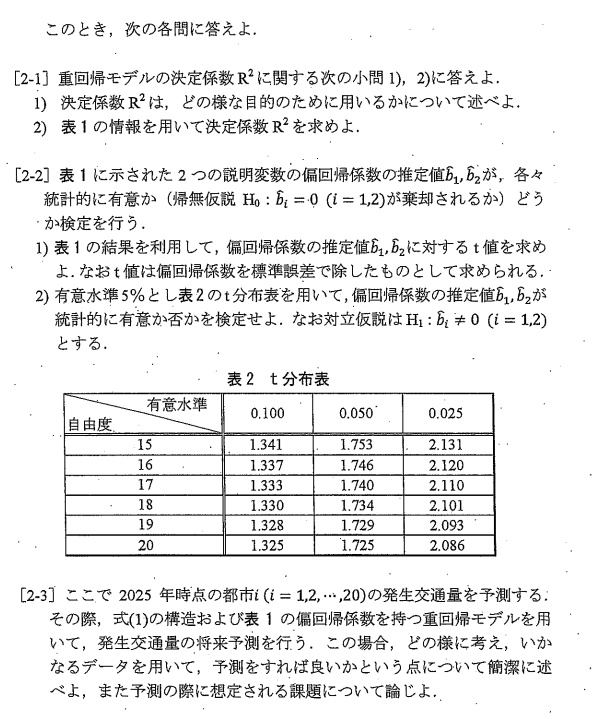
\includegraphics[keepaspectratio, width=16cm]{figures/jyukaiki20133.png}
  \caption{2013年重回帰分析3枚目\label{jyukaiki20133}}
\end{figure}

\pagebreak

[2-1]決定係数$R^2$は独立変数(説明変数)が従属変数(目的変数、被説明変数)のどれくらいを説明できるかを表す値で0から1の値をとります。大きい(1に近い)ほど誤差が少ないことを意味します。決定係数$R^2$は説明変数の数が大きいと1に近づいてしまい予測精度を見誤るという問題もあります。

決定係数$R^2$の定義は1から従属変数の分散(全変動の平方和)と誤差の分散(残差変動の平方和)の比を引いた値です。
$$R^2=\frac{RSS(\textmd{回帰変動平方和})}{TSS\textmd{全変動平方和}}=1-\frac{ESS(\textmd{残差変動平方和})}{TSS(\textmd{全変動平方和})}=1-\frac{\sum_i (y_i-\hat{y}_i)^2}{\sum_i (y_i-\overline{y}_i)^2}$$
従って以下のように求まります。回帰変動の平方和と全変動の平方和の比を用いても同じ解になります。
$$R^2=1-\frac{5.747\times10^6}{1.313\times10^9}=0.995$$

[2-2]求めた係数$b_i$がどの程度予測に寄与しているのかを調べたい場合があります。タイタニック号沈没事故の生存率は性別と階級が生存率に大きく寄与していた(女性を優先して救命ボートに乗せた,下等船室の利用者は見捨てられた)ことが良く知られています。そのような分析を行う場合,各係数$b_i$をその係数の標準偏差で割った値である$t$値で比較します。$t$値は$t$分布に従う確率変数なので帰無仮説(相関が無い仮説)$b_i=0$を両側検定で判別し相関の有意性を調べます。これを$t$検定と呼びます。

$\hat{b_1}$、$\hat{b_2}$に対応する$t$値は偏回帰係数を標準誤差$\sigma_1$,$\sigma_2$で割って以下のように求まります。

\begin{align*}
t_1&=\frac{b_1}{\sigma_1}=\frac{0.353}{0.009}=39.222&t_2&=\frac{b_2}{\sigma_2}=\frac{26.563}{7.379}=3.600
\end{align*}{}

$t$値は対応する自由度の$t$分布と比較します。有意水準$\alpha$なら$|t_i|\ge t_{\alpha/2}(\textmd{自由度})$で帰無仮説$H_0:b_i=0$(有意性がない)を棄却し対立仮説$H_0:b_i\ne0$(有意性がある)を支持します。
自由度$n$は「自由に決めることができる値の数」、「観察値の数から推計値を除いた数」と定義されます。
重回帰分析の$t$値(各$t_i$)の自由度$n$は以下で求められます。
$$n=N(\textmd{標本数})-M(\textmd{説明変数数})-1$$
目的変数$y_i$や説明変数$x_ji$が与えられているとして,偏回帰係数$b_i$を求めるとき「自由に決めることができる値」はN個の誤差$\epsilon_i$だけです。偏回帰係数や決定係数や$t$値は誤差$\epsilon_i$の関数と考えられます。
$$t_i=\textmd{function}(\epsilon_1,\epsilon_2,\cdots,\epsilon_N)$$

但し誤差にも制約条件式があり実は暗黙のうちに誤差について次のような仮定を置いています。

\begin{align*}
\textmd{普遍性(1個):}&\sum_i \epsilon_i=0 
\\
\textmd{等分散性・無相関性(独立性)(M個):}&\sum_i \epsilon_i x_{ji}=0 & (j=1,2,\cdots M\textmd{:説明変数の数})
\end{align*}

従って制約を受けず「自由に決めることができる値の数」即ち自由度$n$は$n=N(\textmd{標本数})-M(\textmd{説明変数数})-1$となるという理解です。
\begin{align*}
\textmd{自由度}n&=20(\textmd{都市数})-2(\textmd{説明変数数})-1=17
\\
有意水準&=\frac{\alpha}{2}=\frac{0.05}{2}=0.025
\end{align*}
より
\begin{align*}
|t_i|\ge t_{0.025}(17\textmd{自由度})=2.110
\end{align*}
を満たせば帰無仮説$H_0:b_i=0$は棄却されます。$\alpha$を2で割っている理由は$t_i$が0より有意に小さい確率$\frac{\alpha}{2}$と0より有意に大きい確率$\frac{\alpha}{2}$を両方考慮に入れるからです。このような検定を両側検定と言います。

この問題では以下のように$b_1$、$b_2$とも有意水準5\%で有意と言えますが$|t_1|\ge |t_2|$より$b_1$の方がより有意と言えます。
\begin{align*}
|t_1|&=39.222\ge2.110&|t_2|&=3.600\ge2.110
\end{align*}

[2-3]どの様に考え,いかなるデータを用いて2025年度の発生交通量を予測すれば良いか、またその場合の課題はというざっくりした問題です。
2025年度の説明変数(夜間人口と商業施設床面積)は2024年現在は観測しようがないので仮定をおいて予測する必要がある点、時間経過により説明変数・被説明変数の関係性が変化し重回帰モデルの適合性が下がる可能性がある点、などを書けば良さそうです。
\end{document}
